\documentclass{report}
\usepackage{cite}
\usepackage{graphicx}
\begin{document}

\title{Electrochemical Biosensor Array Characterization}
\author{Matthew W. Jibson}

\maketitle{}

\pagenumbering{roman}
\setcounter{page}{2}

\begin{abstract}

Advancing our understanding of how the central nervous system works under specific conditions requires real-time, simultaneous detection of a number of key signaling molecules, like nitric oxide (NO). NO diffuses widely and rapidly, has a lifetime in milliseconds, and presents among other high concentration, interfering compounds in the nanomolar range in most biological systems. Current microelectrode-based electrochemical NO sensors have diameters in the micrometer range, much larger than biological cells which are in the micron range, and are thus insufficient for analyzing cell-to-cell interactions. A chip was fabricated using the 0.6$\mu$m CMOS process to overcome these difficulties, with a $5 \times 5$ array of sensors in the 2$\mu$m range. Characterization results of the chip with norepinephrin indicate sensitivity into the 20$\mu$M range and suggest higher-sensitivity devices can offer improvement.

\end{abstract}

\tableofcontents\newpage
\listoffigures\newpage
%\listoftables\newpage

\pagenumbering{arabic}
\setcounter{page}{1}

\chapter{Introduction}

Neurotransmitters play an important role in central nervous systems. Of interest is detecting molecular gradients that are essential in the development of tissue and organ systems. Nitric oxide, a neurotransmitter, is important in this development. Molecular gradients are difficult to detect because of the relative large size of the cells compared to the electrochemical sensors used in sensing systems. Furthermore, in order to detect a gradient, an sensor array must be used in order to collect real-time spatial data. Previous work described the methodology of creating such a sensor array based on CMOS technology. This chip has been fabricated. This paper describes the characterization of the chip in response to expected signals from living cells.

\chapter{Electrochemistry}

Electrochemistry is a process for determining the compounds in a solution. This is accomplished by causing reduction or oxidation within the solution by raising or lowering the potential near some electrode surfaces and measuring the amount of current that is generated.

Specifically, two electrodes are placed into a solution with an electroactive analyte. The potential difference between the electrodes is raised which creates a potential gradient at both electrode-solution interfaces, but a zero potential gradient in the bulk solution between the electrodes. The field strength typically becomes zero at less than $10^{-6}\mathrm{m}$ from the surface of the electrode \cite{kissinger}. When the electroactive analyte nears an electrode, if the potential is high enough, an electron will find favorable conditions in the analyte and transfer from the surface of the electrode to the analyte. At this point there is a concentration gradient between the new, reduced, analyte and the original. The reduced analyte begins to diffuse into the bulk solution, causing more reductions to occur. This happens continuously and at an exponentially decreasing rate until all of the analyte has been reduced. The continuing transfer of electrons causes current to flow. A similar response called oxidation occurs if the potential is lowered and the electron transfers back to the electrode from the analyte. The potential is kept constant by the potentiostat (a device which performs these operations), which measures the current needed to keep the potential constant.

One technique is amperometry, where a constant potential is applied across the electrodes to reduce or oxidize a specific analyte. This technique is able to detect low concentrations and has a fast response time. However, its selectivity is low since all analyte that reduce under the potential applied will also reduce, in addition to the target. Furthermore, the electrodes foul over time, reducing response, and must be cleaned to reproduce results. Electrode surfaces can be made resistive to fouling by applying substances like nafion to the surface.

Another common technique is cyclic voltammetry (CV). Here the potential is swept (at a rate called the scan rate) over a certain range linearly with time, where the range is again dependent on the reduction-oxidation (redox) potential of the analyte. Since both reduction and oxidation potentials are within the range, both occur, and there multiple current spikes in opposite directions. Cyclic voltammetry is useful for determining all of the analytes in a solution since each can present their own current spikes. When the scan rate is high, CV is able to detect analytes that have a short lifetime, like neurotransmitters. High scan rates, however, produce a large background current and thus have a poor limit of detection.

\chapter{Silicon Technology}

The process used in fabricating the chip was the standard 0.6 $\mu$m CMOS process. The CMOS process involves multiple steps that add or remove specific layers of material. To start, a cylindrical (6 inch diameter) ingot of high-purity silicon is created, from which thin (around 500$\mu$m) slices are sawed off called wafers. Chips are square and several milimeters on each side, thus a wafer holds many chips. Due to material and process faults, there are bad areas of the wafer. Chips at these locations do not work, which operational testing is able to determine.

After the wafer is prepared, there were two primary methods used in the CMOS process for this chip: deposition and lithography. Deposition (chemical-vapor deposition, CVD) is a process by which gases or vapors are chemically reacted, leading to the formation of solids on a substrate \cite{microelectronic-circuits}. Common materials for deposition are $\mathrm{SiO_2}$ and $\mathrm{SiNO_3}$. Lithography (also known as photolithography), the second process, is how surface geometry of the various integrated-circuit components is defined. The wafer is coated with a photosensitive layer (called photoresist). A mask will be used to selectively expose the photoresist under ultraviolet light, and the exposed areas will become softened. These areas are then removed using a chemical developer, causing the mask pattern to appear on the wafer.

The simplified fabrication procedure (Fig. \ref{fab-steps}) for the chip began with aluminum being evaporated onto the wafer and patterened using lithography to create probe pads to interface the sensors with the external world, and create contacts and interconnects that carry the sensor current to the probe pads. The chip is deposited with $\mathrm{SiO_2}$ and $\mathrm{SiNO_3}$ to provide insulation between the electrochemical cells and the underlying circuitry. Openings to the probe pads and electrode sites are etched away using lithography. The openings are filled with tungsten to provide contacts between the platinum electrodes and aluminum conductors. The platinum electrodes are fabricated using lithography.

\begin{figure}
\centering
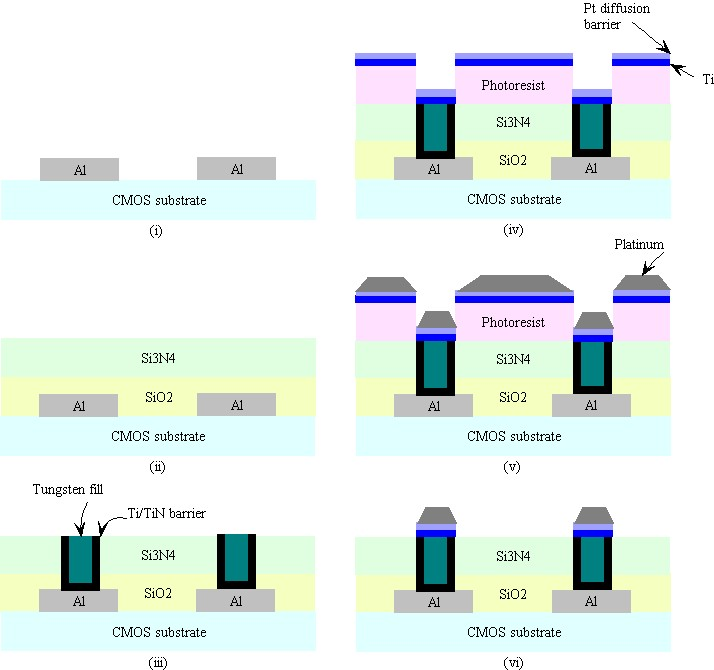
\includegraphics[width=\linewidth]{figures/fabsteps.jpg}
\caption{Fabrication steps and layers.}
\label{fab-steps}
\end{figure}

\chapter{Experimental Setup}

All experiments were done on a Micromanipulator, Inc.\ Probestation. Probe tips and other objects (e.g., pipette tips, thermometer) were held in place by micromanipulators. All electrochemistry experiments were done with a CH Instruments 1207 potentiostat.

Fabrication was done at Avago, Inc., which produced two 6-inch wafers. The wafers were diced by Aspen Technologies to separate the chips. To prepare a single chip, a well of PDMS was constructed such that the exterior would not exceed the edge of the chip and would allow for pins to be lowered onto the probe pads, and the interior would allow the sensor array to be exposed (Fig. \ref{chip-diagram}). This was done so that solution and ovaries could be put over the sensor array with no interference to the probe pads. The well was attached to the chip with glue, producing a seal that would not allow leakage of the interior solution to the probe pads. The well was high enough so that the interior could hold at least 70mL of solution. The interior was wide enough so that ovaries could be easily attached to the surface.

\begin{figure} %{{{ chip-diagram
\centering
\setlength{\unitlength}{0.007 \linewidth}
\begin{picture}(100, 100)
	% 1x1 square
	\newsavebox{\sensor}
	\savebox{\sensor}(1, 1){
		\multiput(0, 0)(0, 1){2}{\line(1, 0){1}}
		\multiput(0, 0)(1, 0){2}{\line(0, 1){1}}
	}

	% 5x5 sensor grid
	\multiput(45, 45.5)(0, 2){5}{\usebox{\sensor}}
	\multiput(47, 45.5)(0, 2){5}{\usebox{\sensor}}
	\multiput(49, 45.5)(0, 2){5}{\usebox{\sensor}}
	\multiput(51, 45.5)(0, 2){5}{\usebox{\sensor}}
	\multiput(53, 45.5)(0, 2){5}{\usebox{\sensor}}

	% vertical pads
	\multiput(0, 0.5)(0, 2){50}{\usebox{\sensor}}
	\multiput(98, 0.5)(0, 2){50}{\usebox{\sensor}}

	% horizontal pads
	\multiput(2, 0.5)(2, 0){48}{\usebox{\sensor}}
	\multiput(2, 98.5)(2, 0){48}{\usebox{\sensor}}

	% exterior
	\multiput(0, 0)(0, 100){2}{\line(100, 0){100}}
	\multiput(0, 0)(100, 0){2}{\line(0, 100){100}}

	% well exterior
	\multiput(2, 2)(0, 96){2}{\line(96, 0){96}}
	\multiput(2, 2)(96, 0){2}{\line(0, 96){96}}

	% well interior
	\put(50, 50){\circle{15}}

	\put(10, 10){probe pads}
	\put(10, 10){\vector(-1, -1){8.5}}

	\put(35, 35){$5 \times 5$ sensor array}
	\put(50, 39){\vector(0, 1){11}}

	\put(35, 65){well interior edge}
	\put(50, 64){\vector(0, -1){6.5}}

	\put(10, 89){well exterior edge}
	\put(25, 93){\vector(0, 1){5}}

	\put(70, 89){chip edge}
	\put(80, 93){\vector(0, 1){7}}
\end{picture}
\caption{Diagram of chip with PDMS well from above.}
\label{chip-diagram}
\end{figure} %}}}

The first characterization of the chip was needed to find the best electrode cell configuration, i.e., the cell with the largest response for a given input. Recall that there are 25 sensor areas. Each area contains multiple working electrodes, and one or more reference and auxiliary electrodes. Two or more working electrodes were tested at each sensor area. Multiple CV runs were performed on each electrode from 0.5V to -0.5V at 0.1V/s in 1M NaCl. The value of an individual run was taken to be the magnitude of the difference of the averages of the two potential sweep directions between -0.2V and 0.2V. That is, the average value from 0.2V to -0.2V in one potential sweep direction was found; the average value from 0.2V to -0.2V in the other potential sweep direction was found; the difference of these averages was found by subtraction. Finally, all results were grouped and averaged per sensor and the sensor area corresponding to the largest result was taken to be the best electrode cell configuration.

To find the ideal potential at which to run the amperometry characterization, a hydrodinamic voltammogram (HDV) was performed to find the optimum potential for amperometry. This was done by running multiple amperometry experiments at identical conditions except for potential, which was varied between 0.6V and 1.25V. In order to ensure identical conditions, the electrode was cleaned before each run by CV from 1.5V to -0.8V at 1V/s for 100 cycles in $\mathrm{H}_2 \mathrm{SO}_4$. The chip well was filled with 50$\mu$L 0.1M KCl. A syringe of 600$\mu$M norepinefrin (NE) was loaded into a pump. The end of the syringe was connected to a pipette, the end of which was lowered into the well so that it was below the surface of the solution. An ameprometry experiment was carried out where the syringe pump would be enabled for 10 seconds at 100$\mu$L/min. The value of the experiment was taken to be the difference between the idle point just before the syringe pump was enabled (generally close to 0) and the lowest point of the resulting curve. The optimum potential was found by taking the largest result.

The final stage of characterization was done to build a find the current generated by a given concentration. This was done using similar conditions as in the HDV characterization. The electrode was cleaned using the CV process with $\mathrm{H}_2 \mathrm{SO}_4$ as listed above. The well was filled with 50$\mu$L 0.1M KCl. A syringe was filled with various concentrations of NE, to which a pipette was connected to the end and lowered into the solution belowe the surface. Amperometry was performed at 0.85V. The syringe pump was enabled for 10 seconds at 100$\mu$L/min after the potentiostat read a stable value close to zero. The value was taken to be the difference between the idle zero point and the lowest point of the resulting curve. This was repeated for each concentration.

Furthermore, the previous experiment was done using both 2 and 4 working electrodes shorted together in parallel (which was possible due to the common reference and auxiliary electrodes for the sensor area we were using). This created a larger effective surface area on the working electrode, theoretically able to sustain a higher current. To verify that this was a valid technique CVs were performed using 100$\mu$M NE in neurobasal (NB) from -0.2V to 1.0V at 0.025V/s. The value was taken to be the lowest recorded point.

Many ovary slices were tested throughout characterization experiments. These were done by preparing a chip with a well and testing it for basic functionality by performing an arbitrary CV. Ovaries were extracted from mice and attached to the surface of the chip over the sensor array, covered in vitrogen. Neurebasal was periodically added to keep the cell from dying and drying out. The ovaries and chips were kept at $37\,^{\circ}\mathrm{C}$ in order to keep them alive. A heat lamp was used during testing with a thermometer measuring temperature directly above the well in an effort to keep the temperature at $37\,^{\circ}\mathrm{C}$. Amperometry tests were run at $0.85V$ for 30 minutes. After the main test, three injections were performed, each of 20$\mu$L: (1) a blank of NB to test for injection noise, (2) 25$\mu$M NE in NB to test the chip's current response to NE, (3) a 1:1 ratio by volume of KCl:NB to release all remaining NE from the cell, which would provide the maximum expected signal from the main 30 minute block.

\chapter{Experimental Results}

Of the 21 different sensor area configurations (numbered 0 - 20), sensor 10 (Fig. \ref{sensor-10} provided the highest average results over the $-0.2V$ to $0.2V$ range. This sensor has common auxiliary and reference electrodes and eight individual working electrodes each $8\mu m$ wide. A similarly good sensor (which ranked first under the range $-0.1V$ to $0.1V$) has a similar configuration, but with working electrodes 10$\mu$m wide.

\begin{figure}
\centering
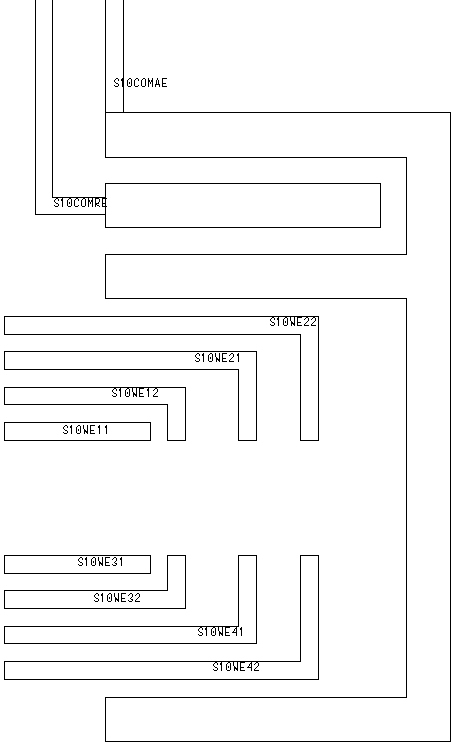
\includegraphics[height=\linewidth]{figures/s10.png}
\caption{Sensor 10 diagram.}
\label{sensor-10}
\end{figure}

The HDV shows the optimum potential for this electrode measuring NE is 0.85V (Fig. \ref{hdv}), which is near the typical value. There is an argument, however, to using a value less than 0.85V in order to decrease noise (other chemicals being reduced), which would also decrease the resulting signal. Since we are already near or perhaps at or limit of detection, though, the added noise is acceptable in order to maximize the output.

\begin{figure}
\centering
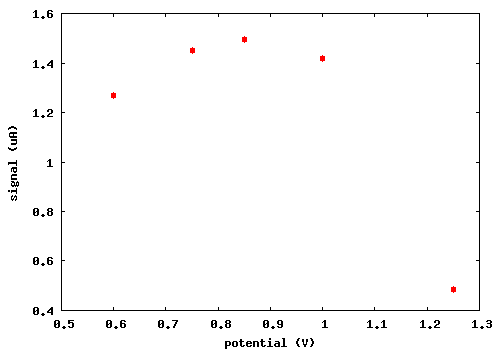
\includegraphics[width=\linewidth]{figures/hdv.png}
\caption{HDV; highest point at $0.85V$.}
\label{hdv}
\end{figure}

Concentration response characterization shows reasonable results in the 25$\mu$M to 200$\mu$M range (Fig. \ref{char}). For 2 pads, the expected output in amperes is $I = C * 2.22604*10^{-12} + 2.28364*10^{-11}$, where $C$ is the molarity of NE. For 4 pads, the expected output in amperes is $I = C * 4.16884*10^{-12} + 2.52294*10^{-11}$, where $C$ is the molarity of NE. As expected, the 4-pad set has a sensitivity slightly less than twice that of the 2-pad set. However, both best-fit lines do not, as expected, cross the origin, and thus suggest a constant amount of background current not dependent on senor area. It is not known---though it is suspected---whether a potentiostat with improved sensitivity (e.g., into the picoamp range) would be able to reliably detect concentrations below 25$\mu$M.

\begin{figure}
\centering
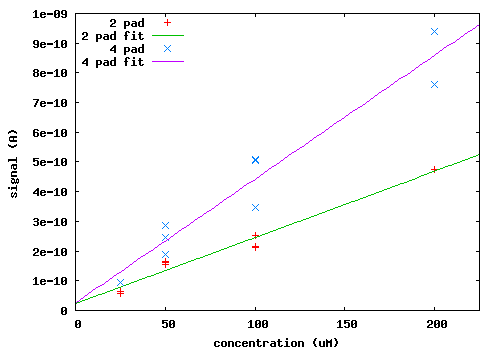
\includegraphics[width=\linewidth]{figures/char.png}
\caption{2- and 4-pad characterizations with 1st order best-fit lines.}
\label{char}
\end{figure}

Ovary test results show our potentiostat is not sensitive enough to detect possible NE releases from the cell. As we expect releases in the nanomolar and subnanomolar range, which we cannot currently detect due to potentiostat limitations, this is expected \cite{amperometry-review}. The three injections at the end of the testing are not statistically differentiable and do not correspond to our expectations of what should occur. It could also mean the chip sensors were damaged or restricted during ovary attachment and cannot function as expected.

\chapter{Conclusion}

We fabricated a chip with an array of electrochemical sensor cells of varying make. This chip was characterized to find high-performing cells, an optimum amperometry potential for these cells, and the response to various concentrations of expected chemicals that would be released by living cells. Further research with highly-sensitive instruments is needed to determine the limit of detection of this chip.

\bibliography{thesis}{}
\bibliographystyle{ieeetr}

\end{document}
